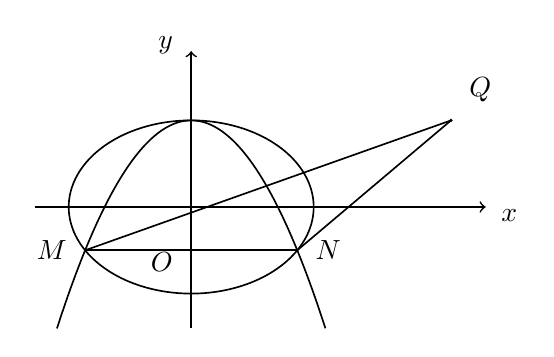
\begin{tikzpicture}[x=1.1cm,y=1.1cm,line width=.6pt]
\draw[->] (-1.8,0) -- (3.4,0) node[below=3pt,right=2pt] {$x$};
\draw[->] (0,-1.4) -- (0,1.8) node[above=2pt,left=3pt] {$y$};
\node[below left=2pt,xshift=-1pt,yshift=-11pt] at (0,0) {$O$};
% ellipse C2: x^2/2+y^2=1
\draw[domain=0:360,samples=160,variable=\t] plot ({1.41421356*cos(\t)},{sin(\t)});
% parabola C1: x^2+y=1 -> y=1-x^2, clip to view
\draw[domain=-1.55:1.55,samples=120] plot (\x,{1-\x*\x});
% points M,N: u=sqrt(3/2)~1.2247, v=-0.5
\coordinate (M) at (-1.22474487,-0.5);
\coordinate (N) at (1.22474487,-0.5);
\coordinate (Q) at (3,1);
\fill (Q) circle (0.02);
\draw (M) -- (N);
\draw (M) -- (Q);
\draw (N) -- (Q);
\node[left=3pt] at (M) {$M$};
\node[right=3pt] at (N) {$N$};
\node[above right=3pt] at (Q) {$Q$};
\end{tikzpicture}
